\documentclass[tikz,border=5mm]{standalone}
\usepackage{tikz}
\usetikzlibrary{calc}

% --- COLOR DEFINITIONS ---
\definecolor{CDark}{HTML}{1F414D}
\definecolor{Garnet}{HTML}{73000A}
\definecolor{CBlue}{HTML}{466A9F}
\definecolor{CGrayLight}{HTML}{F5F5F5}
\definecolor{CGrayDark}{HTML}{444444}
\definecolor{COrange}{HTML}{E07020}

\begin{document}
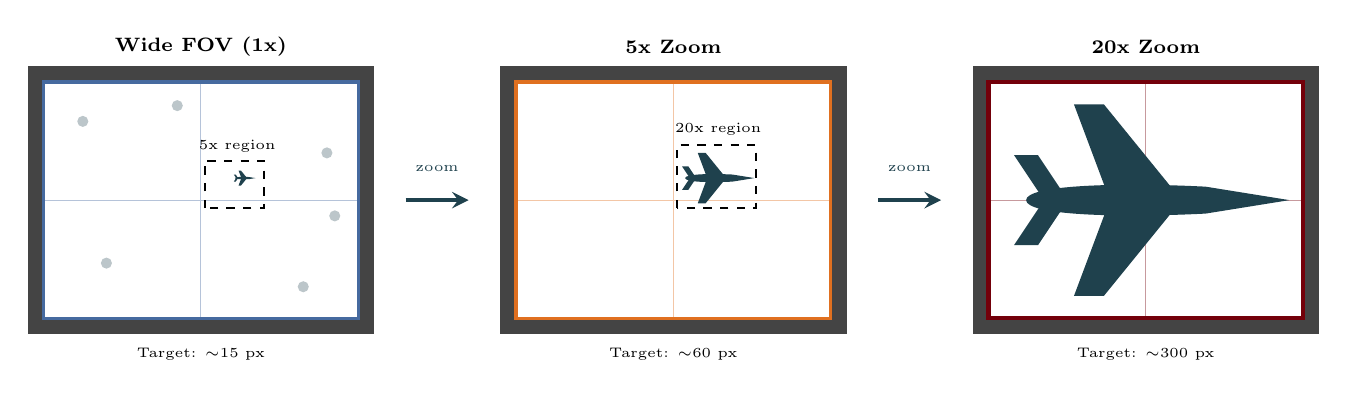
\begin{tikzpicture}

  % ============================================
  % FRAME 1: Wide FOV (1x) - Full scene
  % ============================================
  \begin{scope}[shift={(0,0)}]
    % Frame border (camera housing style)
    \fill[CGrayDark] (-2.2,-1.7) rectangle (2.2,1.7);
    \draw[very thick, CBlue, fill=white] (-2,-1.5) rectangle (2,1.5);
    
    % Crosshairs (subtle)
    \draw[CBlue!40, thin] (-2,0) -- (2,0);
    \draw[CBlue!40, thin] (0,-1.5) -- (0,1.5);
     \draw[very thick, CBlue] (-2,-1.5) rectangle (2,1.5);
    
    % Scattered scene elements (other objects - birds, clouds, etc)
    \foreach \x/\y in {-1.5/1.0, -1.2/-0.8, 1.6/0.6, 1.3/-1.1, -0.3/1.2, 1.7/-0.2} {
      \fill[CDark!30] (\x, \y) circle (2pt);
    }
    
    % === AIRCRAFT AT 1x: Just a small blob/speck ===

    \begin{scope}[shift={(0.55, 0.28)}, scale=0.03]
      % 1. Fuselage - Solid single shape
      \fill[CDark] 
        (-4.0, 0) .. controls (-4.0, 0.5) and (-1, 0.6) .. (2.0, 0.45) % Top edge
        -- (4.8, 0) % Nose
        -- (2.0, -0.45) % Bottom edge
        .. controls (-1, -0.6) and (-4.0, -0.5) .. (-4.0, 0); % Rear
      
      % 2. Main Wings - Start from Centerline to prevent gaps
      \fill[CDark] 
        (0.8, 0) -- (-1.2, 0) -- (-2.4, 3.2) -- (-1.4, 3.2) -- (1.2, 0) -- cycle;
      \fill[CDark] 
        (0.8, 0) -- (-1.2, 0) -- (-2.4, -3.2) -- (-1.4, -3.2) -- (1.2, 0) -- cycle;
      
      % 3. Horizontal Stabilizers (Tail) - Start from Centerline
      \fill[CDark] 
        (-2.6, 0) -- (-3.4, 0) -- (-4.4, 1.5) -- (-3.6, 1.5) -- (-2.6, 0) -- cycle;
      \fill[CDark] 
        (-2.6, 0) -- (-3.4, 0) -- (-4.4, -1.5) -- (-3.6, -1.5) -- (-2.6, 0) -- cycle;


    \end{scope}
    
    
    % 5x zoom region indicator (nested box)
    \draw[black, thick, dashed] (0.05,-0.1) rectangle (0.8,0.5);
    \node[font=\tiny, black, anchor=south west] at (-0.15, 0.48) {5x region};
    
    % Labels
    \node[font=\scriptsize\bfseries, black] at (0, 1.95) {\textbf{Wide FOV (1x)}};
    \node[font=\tiny, black] at (0, -1.95) {Target: $\sim$15 px};
  \end{scope}
  
  % Arrow 1->2
  \draw[->, ultra thick, CDark, >=stealth] (2.6, 0) -- (3.4, 0);
  \node[font=\tiny, CDark, align=center] at (3.0, 0.4) {zoom};

  % ============================================
  % FRAME 2: 5x Zoom - Cropped region  
  % ============================================
  \begin{scope}[shift={(6.0,0)}]
    % Frame border
    \fill[CGrayDark] (-2.2,-1.7) rectangle (2.2,1.7);
    \draw[very thick, COrange, fill=white] (-2,-1.5) rectangle (2,1.5);
    
    % Crosshairs
    \draw[COrange!40, thin] (-2,0) -- (2,0);
    \draw[COrange!40, thin] (0,-1.5) -- (0,1.5);

    \draw[very thick, COrange] (-2,-1.5) rectangle (2,1.5);

    
    % === AIRCRAFT AT 5x: Recognizable silhouette ===

    \begin{scope}[shift={(0.55, 0.28)}, scale=0.10]
      % 1. Fuselage - Solid single shape
      \fill[CDark] 
        (-4.0, 0) .. controls (-4.0, 0.5) and (-1, 0.6) .. (2.0, 0.45) % Top edge
        -- (4.8, 0) % Nose
        -- (2.0, -0.45) % Bottom edge
        .. controls (-1, -0.6) and (-4.0, -0.5) .. (-4.0, 0); % Rear
      
      % 2. Main Wings - Start from Centerline to prevent gaps
      \fill[CDark] 
        (0.8, 0) -- (-1.2, 0) -- (-2.4, 3.2) -- (-1.4, 3.2) -- (1.2, 0) -- cycle;
      \fill[CDark] 
        (0.8, 0) -- (-1.2, 0) -- (-2.4, -3.2) -- (-1.4, -3.2) -- (1.2, 0) -- cycle;
      
      % 3. Horizontal Stabilizers (Tail) - Start from Centerline
      \fill[CDark] 
        (-2.6, 0) -- (-3.4, 0) -- (-4.4, 1.5) -- (-3.6, 1.5) -- (-2.6, 0) -- cycle;
      \fill[CDark] 
        (-2.6, 0) -- (-3.4, 0) -- (-4.4, -1.5) -- (-3.6, -1.5) -- (-2.6, 0) -- cycle;


    \end{scope}
    
    % 20x zoom region indicator (nested box)
    \draw[black, thick, dashed] (0.05,-0.1) rectangle (1.05,0.7);
    \node[font=\tiny, black, anchor=south west] at (-0.1, 0.7) {20x region};
    
    % Labels
    \node[font=\scriptsize\bfseries, black] at (0, 1.95) {\textbf{5x Zoom}};
    \node[font=\tiny, black] at (0, -1.95) {Target: $\sim$60 px};
  \end{scope}
  
  % Arrow 2->3
  \draw[->, ultra thick, CDark, >=stealth] (8.6, 0) -- (9.4, 0);
  \node[font=\tiny, CDark, align=center] at (9.0, 0.4) {zoom};

  % ============================================
  % FRAME 3: 20x Zoom - Maximum detail
  % ============================================
  \begin{scope}[shift={(12.0,0)}]
    % Frame border (emphasized)
    \fill[CGrayDark] (-2.2,-1.7) rectangle (2.2,1.7);
    \draw[ultra thick, Garnet, fill=white] (-2,-1.5) rectangle (2,1.5);
    
    % Fine crosshairs with tick marks
    \draw[Garnet!40, thin] (-2,0) -- (2,0);
    \draw[Garnet!40, thin] (0,-1.5) -- (0,1.5);

    \draw[ultra thick, Garnet] (-2,-1.5) rectangle (2,1.5);
    
    % === AIRCRAFT AT 20x: Full detail ===
    \begin{scope}[shift={(0, 0)}, scale=0.38]
      % 1. Fuselage - Solid single shape
      \fill[CDark] 
        (-4.0, 0) .. controls (-4.0, 0.5) and (-1, 0.6) .. (2.0, 0.45) % Top edge
        -- (4.8, 0) % Nose
        -- (2.0, -0.45) % Bottom edge
        .. controls (-1, -0.6) and (-4.0, -0.5) .. (-4.0, 0); % Rear
      
      % 2. Main Wings - Start from Centerline to prevent gaps
      \fill[CDark] 
        (0.8, 0) -- (-1.2, 0) -- (-2.4, 3.2) -- (-1.4, 3.2) -- (1.2, 0) -- cycle;
      \fill[CDark] 
        (0.8, 0) -- (-1.2, 0) -- (-2.4, -3.2) -- (-1.4, -3.2) -- (1.2, 0) -- cycle;
      
      % 3. Horizontal Stabilizers (Tail) - Start from Centerline
      \fill[CDark] 
        (-2.6, 0) -- (-3.4, 0) -- (-4.4, 1.5) -- (-3.6, 1.5) -- (-2.6, 0) -- cycle;
      \fill[CDark] 
        (-2.6, 0) -- (-3.4, 0) -- (-4.4, -1.5) -- (-3.6, -1.5) -- (-2.6, 0) -- cycle;


    \end{scope}
    
    
    % Labels
    \node[font=\scriptsize\bfseries, black] at (0, 1.95) {\textbf{20x Zoom}};
    \node[font=\tiny, black] at (0, -1.95) {Target: $\sim$300 px};
  \end{scope}

\end{tikzpicture}
\end{document}
